\section{Desktop/cleanstuff/i-team/trunk/globals.h File Reference}
\label{globals_8h}\index{Desktop/cleanstuff/i-team/trunk/globals.h@{Desktop/cleanstuff/i-team/trunk/globals.h}}
Holds the names of the global variables used throughout all the game code. 

{\tt \#include \char`\"{}library\_\-h/gp2d.h\char`\"{}}\par
{\tt \#include \char`\"{}players.h\char`\"{}}\par
{\tt \#include \char`\"{}weapons.h\char`\"{}}\par
{\tt \#include \char`\"{}functions.h\char`\"{}}\par
{\tt \#include \char`\"{}mainmenu.h\char`\"{}}\par
{\tt \#include \char`\"{}basicwidget.h\char`\"{}}\par
{\tt \#include \char`\"{}settings.h\char`\"{}}\par
{\tt \#include \char`\"{}iteam\_\-maths.h\char`\"{}}\par


Include dependency graph for globals.h:\nopagebreak
\begin{figure}[H]
\begin{center}
\leavevmode
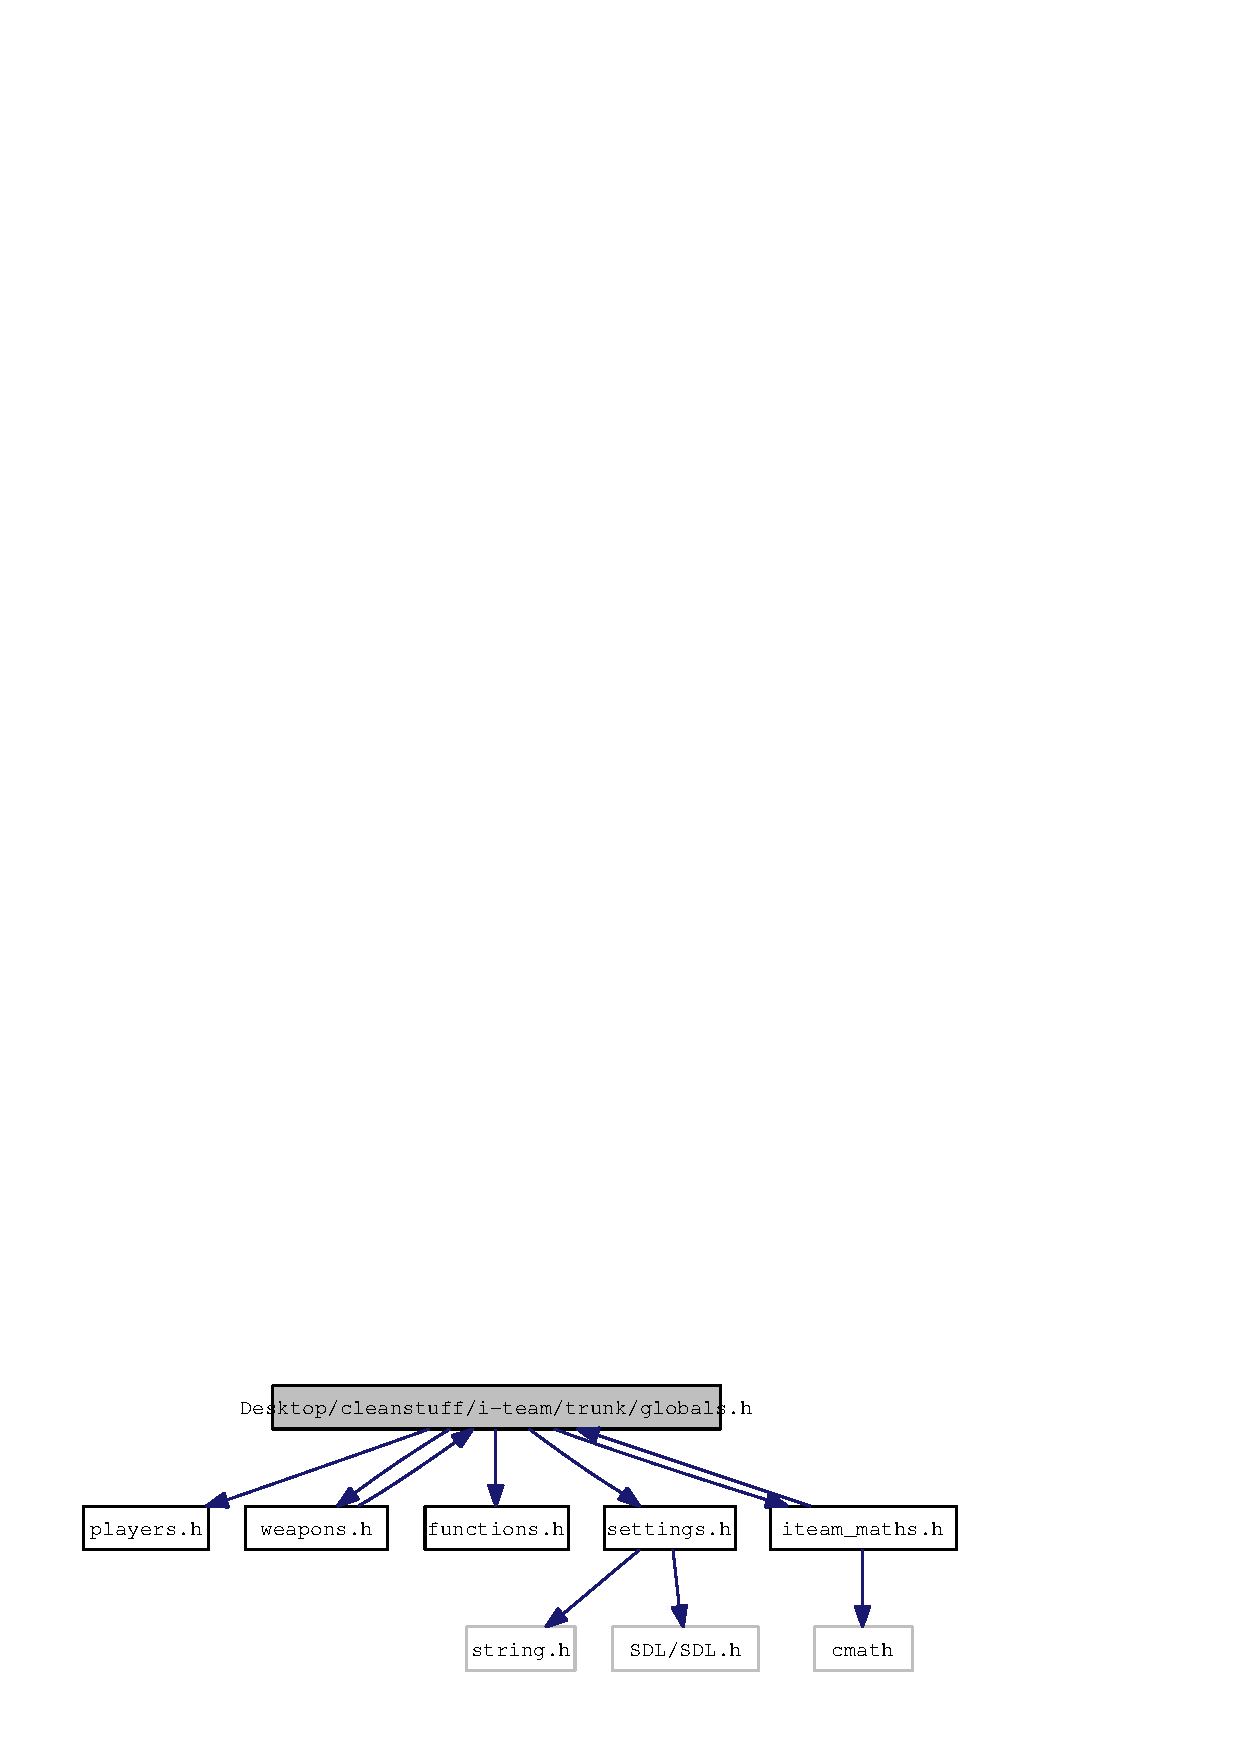
\includegraphics[width=231pt]{globals_8h__incl}
\end{center}
\end{figure}


This graph shows which files directly or indirectly include this file:\nopagebreak
\begin{figure}[H]
\begin{center}
\leavevmode
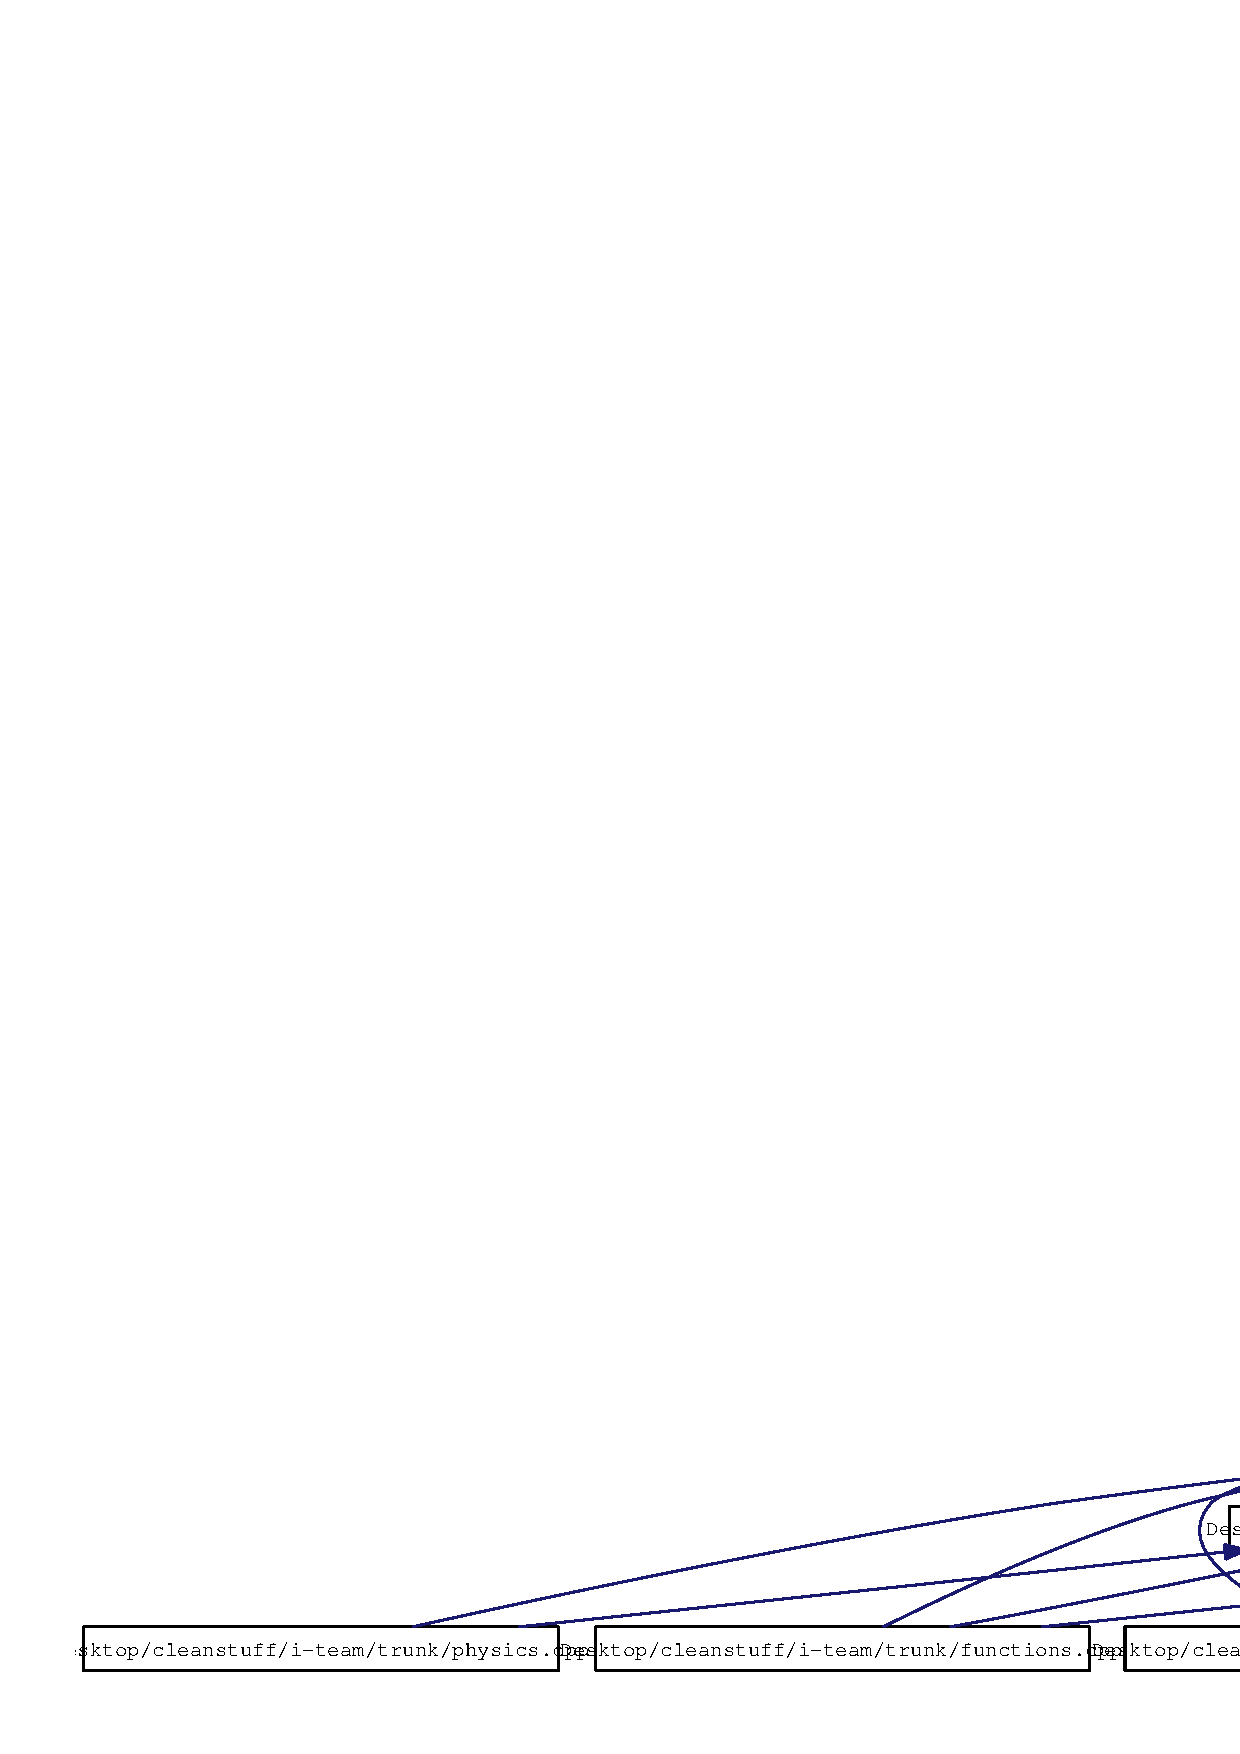
\includegraphics[width=420pt]{globals_8h__dep__incl}
\end{center}
\end{figure}
\subsection*{Namespaces}
\begin{CompactItemize}
\item 
namespace {\bf iteam}
\end{CompactItemize}
\subsection*{Defines}
\begin{CompactItemize}
\item 
\#define {\bf IT\_\-PLAYER\_\-SUSI}~1
\item 
\#define {\bf IT\_\-PLAYER\_\-FACE\_\-LEFT}~true
\item 
\#define {\bf IT\_\-PLAYER\_\-FACE\_\-RIGHT}~false
\item 
\#define {\bf THUMBS\_\-WIDTH}~284
\item 
\#define {\bf THUMBS\_\-HEIGHT}~28
\end{CompactItemize}
\subsection*{Variables}
\begin{CompactItemize}
\item 
vector$<$ iteam::PlayerObj $>$ {\bf iteam::Player}
\item 
gp2d::Sprite {\bf iteam::Tank\_\-base}
\item 
gp2d::Sprite {\bf iteam::Tank\_\-canon}
\item 
gp2d::Sprite {\bf iteam::AnglePointer}
\item 
gp2d::Sprite {\bf iteam::WeaponSelector}
\item 
gp2d::Camera {\bf iteam::Cam}
\item 
int {\bf iteam::GameResW}
\item 
int {\bf iteam::GameResH}
\item 
int {\bf iteam::CurPlayer}
\item 
int {\bf iteam::CountdownValue}
\item 
bool {\bf iteam::GameRunning}
\item 
gp2d::Timer {\bf iteam::iTimer}
\item 
int {\bf iteam::CurrentWeapon} = IT\_\-WT\_\-GRENADE
\item 
gp2d::inputHandler $\ast$ {\bf KeyHandler}
\end{CompactItemize}


\subsection{Detailed Description}
Holds the names of the global variables used throughout all the game code. 

This is just a bunch of \char`\"{}extern\char`\"{} variable declarations... they are a \char`\"{}fake\char`\"{} image of the real variables. It will tell the compiler that the variable exists and to not to search for it. Thus, we need to re-declare that variable. Most of the variables declared as extern in Globals.h are really declared at iteam.cpp 

\subsection{Define Documentation}
\index{globals.h@{globals.h}!IT_PLAYER_FACE_LEFT@{IT\_\-PLAYER\_\-FACE\_\-LEFT}}
\index{IT_PLAYER_FACE_LEFT@{IT\_\-PLAYER\_\-FACE\_\-LEFT}!globals.h@{globals.h}}
\subsubsection{\setlength{\rightskip}{0pt plus 5cm}\#define IT\_\-PLAYER\_\-FACE\_\-LEFT~true}\label{globals_8h_4c84f21a52a1f443f99171f15a756e35}


Boolean flag for the Mirror property of a GP2D::Sprite. This is just so it can be read easier on the code rather than true/false and not knowing which direction the player is facing \index{globals.h@{globals.h}!IT_PLAYER_FACE_RIGHT@{IT\_\-PLAYER\_\-FACE\_\-RIGHT}}
\index{IT_PLAYER_FACE_RIGHT@{IT\_\-PLAYER\_\-FACE\_\-RIGHT}!globals.h@{globals.h}}
\subsubsection{\setlength{\rightskip}{0pt plus 5cm}\#define IT\_\-PLAYER\_\-FACE\_\-RIGHT~false}\label{globals_8h_37ceb0d034894db890e9bd4f47760acc}


Boolean flag for the Mirror property of a GP2D::Sprite. This is just so it can be read easier on the code rather than true/false and not knowing which direction the player is facing \index{globals.h@{globals.h}!IT_PLAYER_SUSI@{IT\_\-PLAYER\_\-SUSI}}
\index{IT_PLAYER_SUSI@{IT\_\-PLAYER\_\-SUSI}!globals.h@{globals.h}}
\subsubsection{\setlength{\rightskip}{0pt plus 5cm}\#define IT\_\-PLAYER\_\-SUSI~1}\label{globals_8h_1da2d4ad7659310cbe68fb0f54a58cde}


Susi's ID, code-wise: 1. See an example of this in Players.cpp/.h \index{globals.h@{globals.h}!THUMBS_HEIGHT@{THUMBS\_\-HEIGHT}}
\index{THUMBS_HEIGHT@{THUMBS\_\-HEIGHT}!globals.h@{globals.h}}
\subsubsection{\setlength{\rightskip}{0pt plus 5cm}\#define THUMBS\_\-HEIGHT~28}\label{globals_8h_3278ea0ed112d2a99b5c7e215276adb8}


Height of the inventory relative to the bottom of the screen \index{globals.h@{globals.h}!THUMBS_WIDTH@{THUMBS\_\-WIDTH}}
\index{THUMBS_WIDTH@{THUMBS\_\-WIDTH}!globals.h@{globals.h}}
\subsubsection{\setlength{\rightskip}{0pt plus 5cm}\#define THUMBS\_\-WIDTH~284}\label{globals_8h_bdc4212fc051e4e450e545c220f2fa40}


X start position of the inventory 

\subsection{Variable Documentation}
\index{globals.h@{globals.h}!KeyHandler@{KeyHandler}}
\index{KeyHandler@{KeyHandler}!globals.h@{globals.h}}
\subsubsection{\setlength{\rightskip}{0pt plus 5cm}gp2d::inputHandler$\ast$ {\bf KeyHandler}}\label{globals_8h_e1386f580f80c77ed1a02d791b6b77f4}


This is the global system to handle all key inputs to the game $>$ 